\section*{Grupo 1 - Cluedo matemático (21/11/2016)}

El primer grupo está formado por:
\begin{itemize}
\item Ana Reyes Camacho 

\item Antonio Jesús Guerrero Lobato 

\item Clara Rocío Lambas Magron 

\item Manuel Pulido Lopez 
\end{itemize}
\begin{figure}[h]
\centering
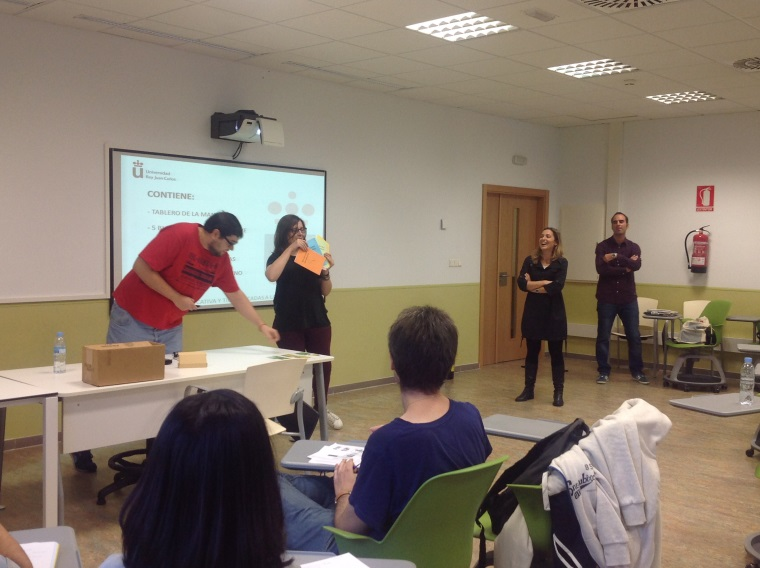
\includegraphics{img/cluedo1.jpg}
\end{figure}
La exposición estaba contextualizada en una clase para alumnos de 1º de la ESO de un IES el último día de clase antes de las vacaciones de Navidad. Durante la clase se tratará la unidad didáctica de la divisibilidad de los números primos y compuestos según aparece en el BOCM. Esta unidad didáctica suele generar mucha confusión entre los alumnos de la ESO y el grupo expositor considera que puede ser de gran interés para el alumnado.

Durante la clase se realizará un juego en el que se formarán varios equipos. Se trata de responder a una serie de preguntas en las que se premiará la rapidez en las respuestas siempre y cuando sean correctas. Por un lado el juego permitirá captar la atención de los alumnos. Por otro, el trabajo en equipo fomenta los valores de colaboración con los compañeros y el hecho de que sean preguntas cronometradas permitirá a las alumnas adaptarse a condiciones de trabajo de ciertas “presión”.

El juego se titula “Cluedo matemático”. El enunciado del juego dice así:

¡Esta noche el Señor Cero ha sido hallado asesinado en su mansión! Los detectives privados Simple y Compuesto han encontrado 99 sospechosos, pero no han podido resolver el caso. ¡Así que ahora la resolución del crimen depende de vosotros! Para ganar el juego debéis averiguar una sola cosa sobre el crimen”

Para la preparación del juego se:
\begin{itemize}
\item[1.] Coloca el tablero, hay un Hall donde empieza la acción y donde se coloca el peón, y 5 habitaciones dónde buscar pistas.

\item[2.] Prepara las tarjetas de preguntas, un tema para cada habitación.

 \item[3.] Prepara las tarjetas de pistas para descubrir al asesino, un pack de pistas por cada equipo.

\item[4.] Organiza a los alumnos en grupo, nombrando un portavoz
\end{itemize}

 \begin{figure}[h]
 \centering
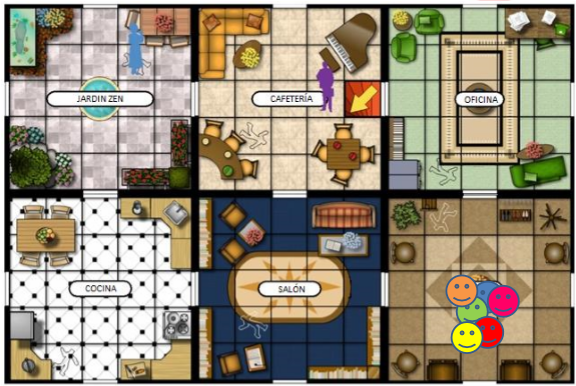
\includegraphics[scale=0.6]{img/cluedo2.jpg}
\end{figure}

Las reglas del juego son:
\begin{itemize}
\item[1.] CÓMO GANAR: ¡Resuelve el crimen!  

\item[2.] CÓMO JUGAR: En cada turno se mueve el peón a una habitación contigua, se le hace a todos los grupos la misma pregunta, se dejan 120'' para calcular la respuesta y si contestan correctamente se les da una pista sobre el asesino.

\begin{figure}[h]
\centering
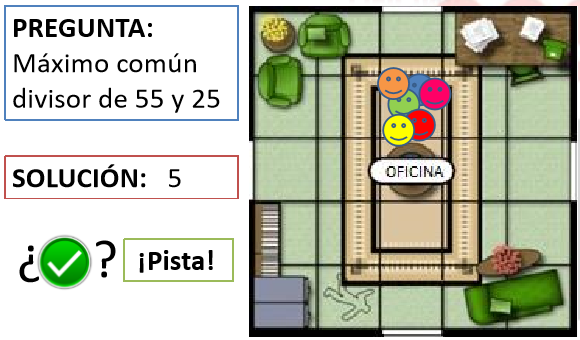
\includegraphics[scale=0.6]{img/cluedo3.jpg}
\end{figure}

\end{itemize}

 
La función principal del juego consistía en hacer preguntas por grupos y había que averiguar el número comprendido entre el 1 y el 99 a partir de una serie de pistas que se iban consiguiendo.

La exposición del grupo estuvo muy bien estructurada y demostraron que hicieron un gran trabajo de equipo.

Durante la misma explicaron que desestimaron la opción de tirar un dado, pero nosotros sí lo habríamos incluido incluyendo la posibilidad de que hubiese un rebote al tener un cronometro. Pero la opción del rebote también la descartaron.

La dificultad de las preguntas era variable por lo que es un juego muy versátil y de alto valor añadido para el aprendizaje.

Nos sorprendieron con algo novedoso al proponer analizar y evaluar el juego al final de la clase, lo que les permitirá que hubiese una mejora continua con los años. Para esta evaluación pidieron a los alumnos que contestaran a una serie de preguntas sobre lo que les ha parecido. Aunque sabemos que es difícil discernir cuando la exposición la realizas en el contexto de alumnos de secundario o en el contexto nuestro de alumnos de master, bajo nuestro punto de vista quizá sea demasiado pronto pedir la opinión a un niño de 1º de la ESO su opinión.

La exposición se ha ajustado perfectamente a los tiempos programados.

\newpage
\section*{Grupo 2 - Construyendo las matemáticas (21/11/2016)}


El segundo grupo está formado por:
\begin{itemize}
\item Helena Matesanz Marín 

\item Cristina Martínez Gonzalez 

\item Eliseo Virseda Alvaro 

\item Noemi Castillo Cumplido 

\item David Soria Castro 
\end{itemize}

\begin{figure}[hbtp]
\centering
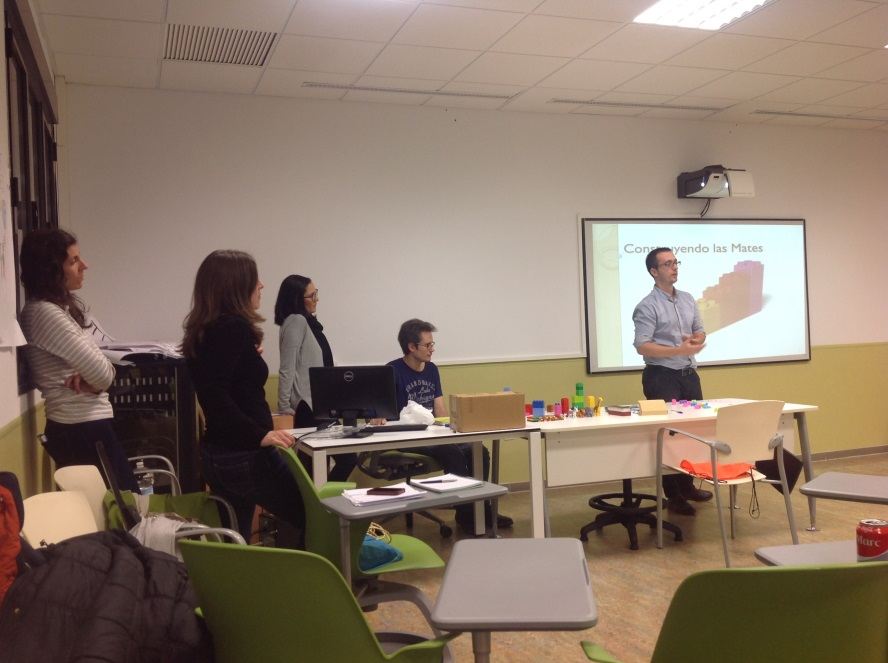
\includegraphics[scale=1]{img/lego1.jpg}
\caption{Integrantes del grupo 2.}
\end{figure}

 
La exposición consistió en explicar con un material manipulativo conocido por los alumnos, que son las piezas de LEGO, los siguientes conceptos matemáticos que en el papel pueden parecer abstractos. Los conceptos matemáticos mostrados fueron:
\begin{itemize}
\item Fracciones 

\item Estadística 

\item Máximo común divisor y mínimo común múltiplo 

\item Ecuaciones lineales simples. Despejar la x. 

\item Teorema de Pitágoras 
\end{itemize}

\begin{figure}[hbtp]
\centering
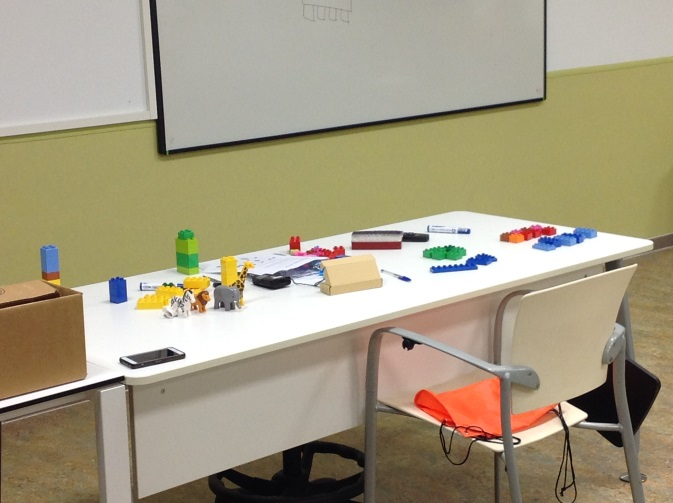
\includegraphics[scale=1]{img/lego2.jpg}
\caption{Materiales manipulativos.}
\end{figure}
 
En nuestra opinión el uso de LEGO para varios conceptos matemáticos hizo que algunos de estos temas estuvieran un poco forzados. Es decir, para el concepto de fracciones las piezas de LEGO fueron de gran utilidad al permitir de una manera visual entender el concepto de lo que es una fracción como una parte de un todo. Sin embargo consideramos que explicar el concepto de M.c.d y m.c.m con piezas de LEGO quedó un poco forzado.

Por hacer una crítica constructiva, entendemos que era un grupo de 5 alumnos, es decir, de más alumnos que el resto de grupos de clase, pero quizá hubiésemos enfocado el trabajo en uno o dos conceptos matemáticos y habríamos trabajado un par de alumnos por cada concepto para evitar explicaciones de conceptos forzadas.

La exposición estuvo muy bien estructurada con una demostración conceptual por cada alumno pero se fueron de tiempo. Es cierto que se han explicado muchos conceptos pero los alumnos no hemos colaborado con lo que se puede perder eficacia al no hacer partícipes a los alumnos. Pero también entendemos que todos tenían que hablar y que eran temas muy interesantes.

Por último, la exposición también nos sirvió para aprender que a día de hoy hay un software en una web de internet (\url{http://www.publishyourdesign.com/}) que te permite realizar diseños de LEGO en 3D con el ordenador para luego poder incluso imprimirlos con impresoras 3D.

\newpage
\section*{Grupo 4 - La Oca Matemática (28/11/2016)}

Integrantes del grupo:

\begin{itemize}

\item Óscar Abelda
\item Miriam Expósito
\item Beatriz Mate
\item Pablo Saiz
\end{itemize}

\begin{minipage}[hbtp]{1.0\linewidth}
\centering
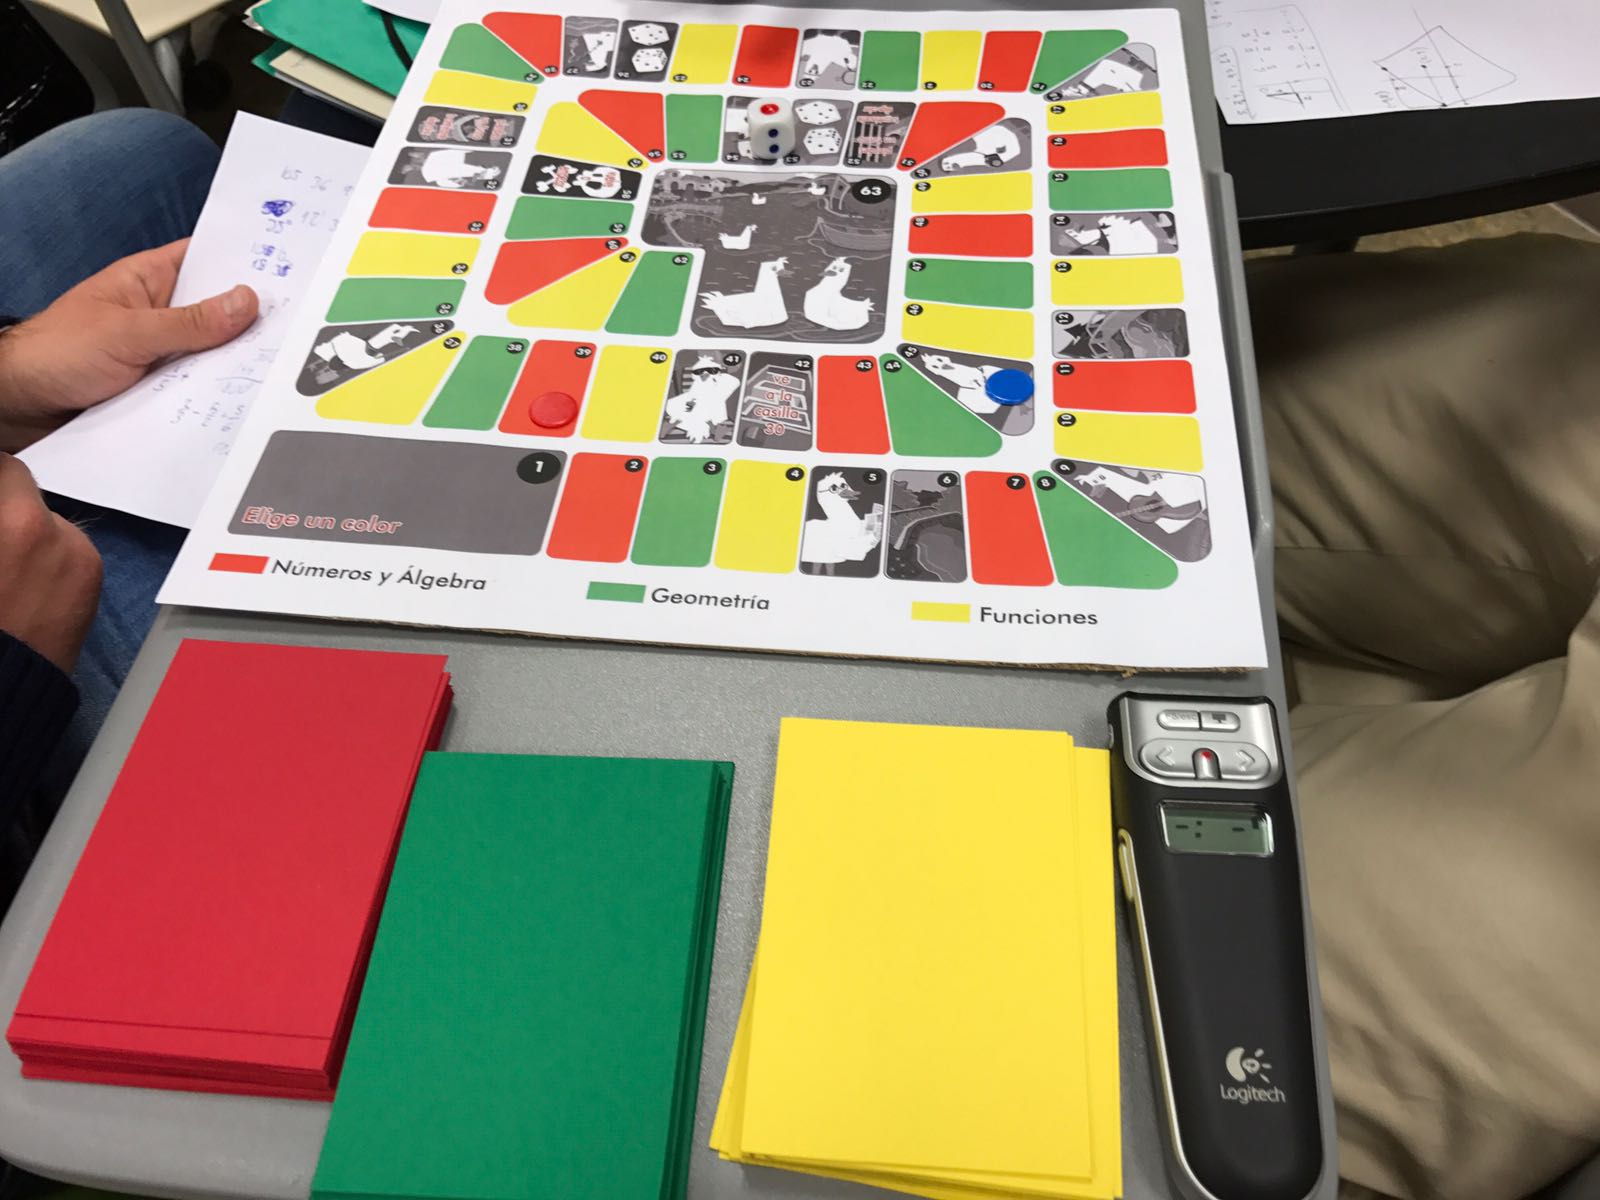
\includegraphics[scale=0.2]{img/grupo4_1.jpg}
\captionof{figure}{Material para cada grupo}.
\end{minipage}

Se presentó un juego clásico rediseñado para su aplicación en el campo de las matemáticas de 2º de la ESO. Desde un principio han sido capaces de meternos en el contexto de la situación en la cual sería aplicable la actividad. Está orientada a ese último día de clase donde podemos repasar contenidos de forma lúdica, sin que resulte aburrido para el alumnado. 

Nos sorprendió gratamente el gran trabajo realizado a la hora de elaborar el material manipulativo. La actividad contenía las instrucciones del juego, dado, tablero, tarjetas de contenidos, fichas, etc. Estábamos ante un juego de sobremesa con todo tipo de detalles.

Al poco tiempo de comenzar el juego, nos dimos cuenta de que pese a nuestra edad, poco a poco se iba incrementando la competitividad entre nosotros. No parábamos de comprobar si la pareja opuesta estaba resolviendo bien las preguntas, tiempo empleado, cuáles eran sus materias fuertes, etc. En todo momento contamos con un supervisor del grupo autor del juego, que nos guió durante la actividad.


\newpage
\section*{Grupo 5 - Pasapalabra-Pitágoras}

El grupo está formado por:

\begin{itemize}
\item Noelia Díaz Concepción
\item Borja González Blasco
\item Raquel Navas Sánchez
\item Carlos Rodiño Lourenco
\end{itemize}

Este grupo ha realizado su presentación mediante un recurso educativo de los que vimos en clase, el video, lo cual nos pareció muy interesante ya que de esta forma mostraron la utilidad de dicho recurso. 

Su trabajo de innovación se centra en una clase de primero de la E.S.O, en concreto, en la explicación del teorema de Pitágoras. En primer lugar definen las partes del teorema a través del juego de televisión de Pasapalabra. Después de esta parte introductoria, su trabajo se centra en la realización de tres tareas: la primera de ellas tiene como objetivo demostrar el teorema y las otras dos son para aplicar los conocimientos aprendidos del teorema. A continuación se muestra cada una de ellas.

\begin{itemize}

\item Actividad 1: Demostración que el cuadrado de la hipotenusa es igual a la suma del cuadrado de los catetos. Para ello se necesitan pajitas, tijeras, celo y garbanzos. 

\begin{figure}[hbtp]
\centering
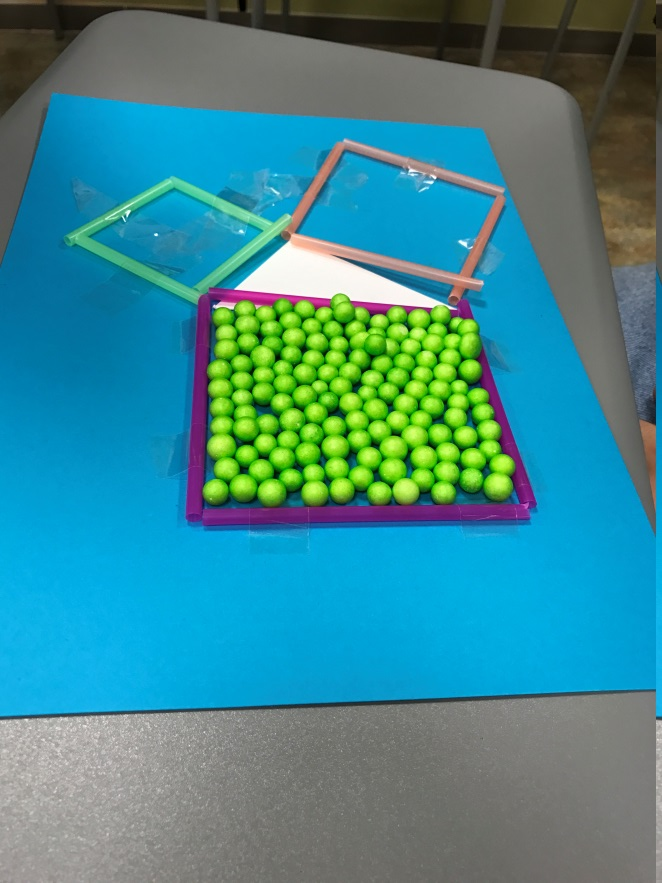
\includegraphics{img/grupo5_1.jpg}
\caption{Actividad 1}
\end{figure}



\item Actividad 2: Aplicación del teorema para obtener el camino que tiene que seguir el conejo: uso de calculadora. El ganador de esta actividad recibe unas monedas de chocolate

\begin{figure}[hbtp]
\centering
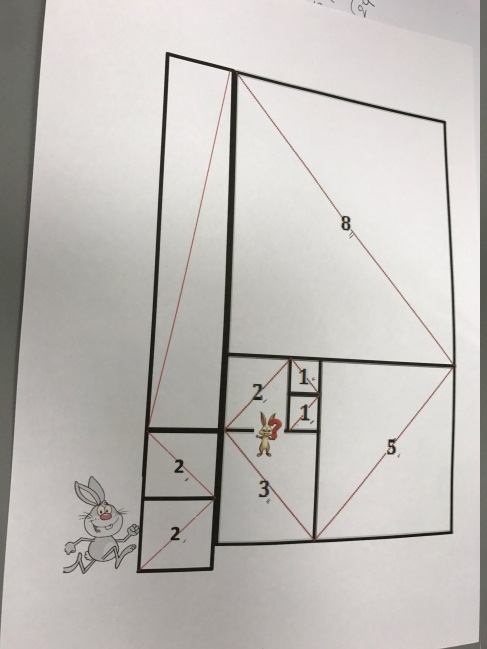
\includegraphics{img/grupo5_2.jpg}
\caption{Actividad 2}
\end{figure}


\item Actividad 3: Aplicación del teorema en un edificio: sin usar la calculadora. El ganador de esta actividad recibe una tableta de chocolate. 

\begin{figure}[hbtp]
\centering
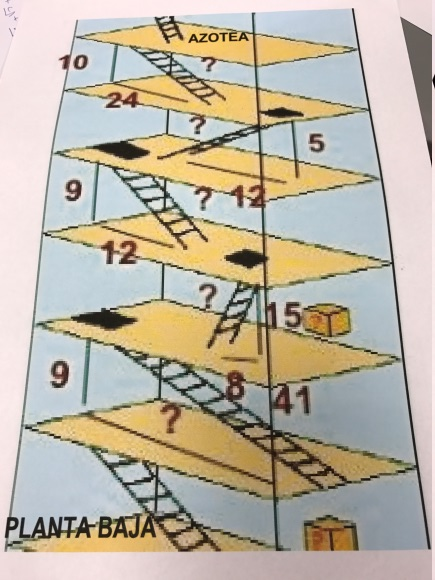
\includegraphics{img/grupo5_3.jpg}
\caption{Actividad 3}
\end{figure}

\end{itemize}

Nos ha parecido una actividad muy completa ya que utiliza diferentes recursos: vídeo, matemáticas recreativas mediante los juegos y manipulativa mediante el uso de las pajitas y garbanzos para demostrar el teorema. El hecho de introducir un premio después de las actividades de aplicación nos ha parecido una idea interesante y que además ninguno habíamos usado. Nos parece una gran forma de motivar e ilusionar a los estudiantes para que hagan la actividad de la mejor forma y lo más rápido posible, fomentando así mismo una competitividad sana. Nos ha gustado mucho el uso del vídeo y muy práctico. En general, nos ha parecido un gran trabajo y bastante divertido.


\newpage
\section*{Grupo 6 - Triangulo de Sierpinski}

El grupo 6 está formado por:

\begin{itemize}

\item Maria Rosa Calvo Arrojo 

\item Victor Fernandez Alcala 

\item Emilio Jose Hernandez Rodriguez 

\item José Miguel Hernando Santacruz 
\end{itemize}

El trabajo de innovación de este grupo se centra en una clase de tercero de la E.S.O. en el apartado de números y algebra, más concretamente en la explicación del tema de sucesiones. Su trabajo se divide en 4 partes y cada componente del grupo explica una de ellas. En primer lugar, nos muestran diferentes tipos de verdura para estudiar como hay una unidad que se repite, que es lo que se conoce como fractales. Su idea es que los alumnos al ver las verduras averigüen qué forma se está repitiendo en cada caso. Una vez averiguado se explica un poco la historia sobre este apartado para después comenzar con la explicación concreta del triángulo de Sierpinski.


\begin{figure}[hbtp]
\centering
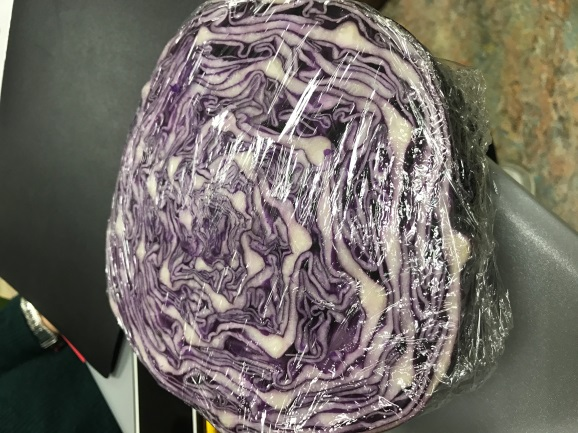
\includegraphics[scale=1.2]{img/grupo6_1.jpg}
\end{figure}


En esta segunda parte, proporcionan material manipulativo (goma eva, cartulinas) para que se trabaje con él y se entienda mejor el concepto de repeticiones que están explicando. A continuación se muestra el resultado de las distintas actividades realizadas:



\begin{figure}[h]
\centering
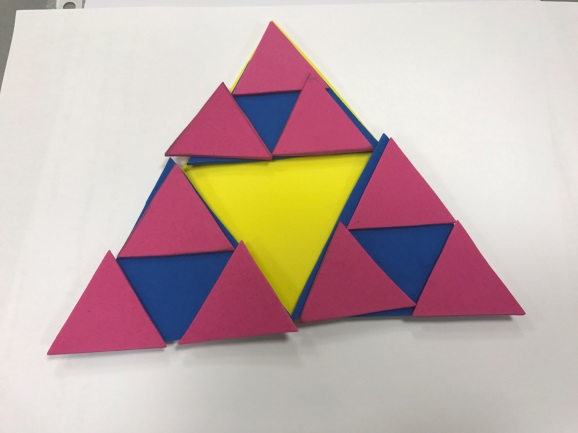
\includegraphics{img/grupo6_2.jpg}
\caption{Triángulo de Sierpinski construido con materiales manipulativos.}
\end{figure}

\begin{figure}[h]
\centering
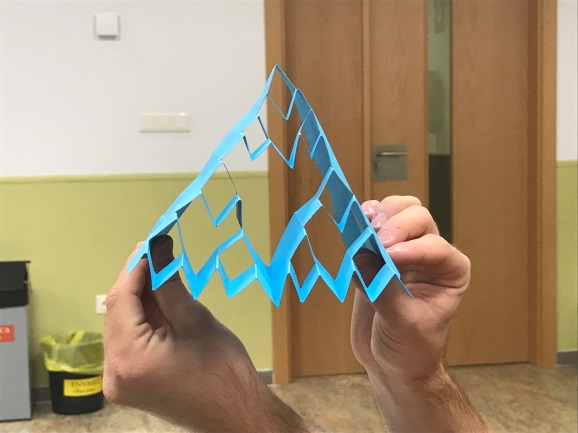
\includegraphics{img/grupo6_3.jpg}
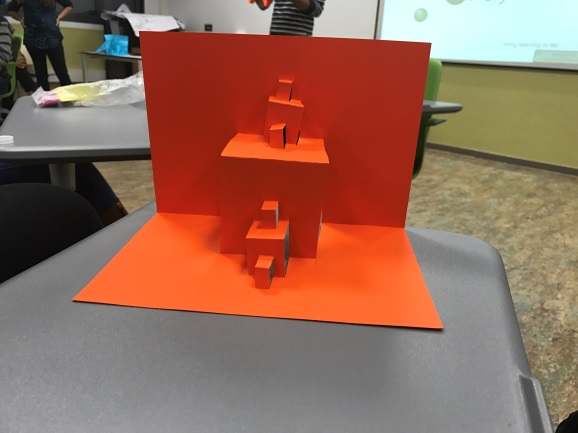
\includegraphics{img/grupo6_4.jpg}
\end{figure}



Finalmente y una vez trabajado con el material proporcionado, se realiza la explicación en sí de las sucesiones.

Lo que más nos ha gustado de este trabajo es la posibilidad de trabajar con material manipulativo, siendo especialmente chulo e interesante las formas que se obtienen con el trabajo sobre las cartulinas. Quizás se ha echado en falta más material para que todos los alumnos puedan trabajar y realizar esas formas ya que la mejor forma de entusiasmar a los alumnos y hacer que estos estén pendientes de la explicación es que todos puedan trabajar con sus propias manos en lugar de observar. Por otro lado nos ha parecido muy interesante el hecho de realizar una conexión entre el tema matemático a tratar y la vida real, a través de la demostración de la forma de crecimiento de las verduras. Finalmente, les ha faltado incluir una hoja de valoraciones en su trabajo para que sepan las opiniones de los distintos grupos y las posibles mejoras que podrían aplicar en su trabajo de innovación.


\newpage
\section*{Grupo 7 - Clase de repaso 4º ESO B (académicas)}

El séptimo grupo está formado por:

\begin{itemize}
\item Lourdes Fuentes
\item Pedro Juan Valle
\item Daniel Camarero
\item David García
\end{itemize}


\begin{figure}[h]
\centering
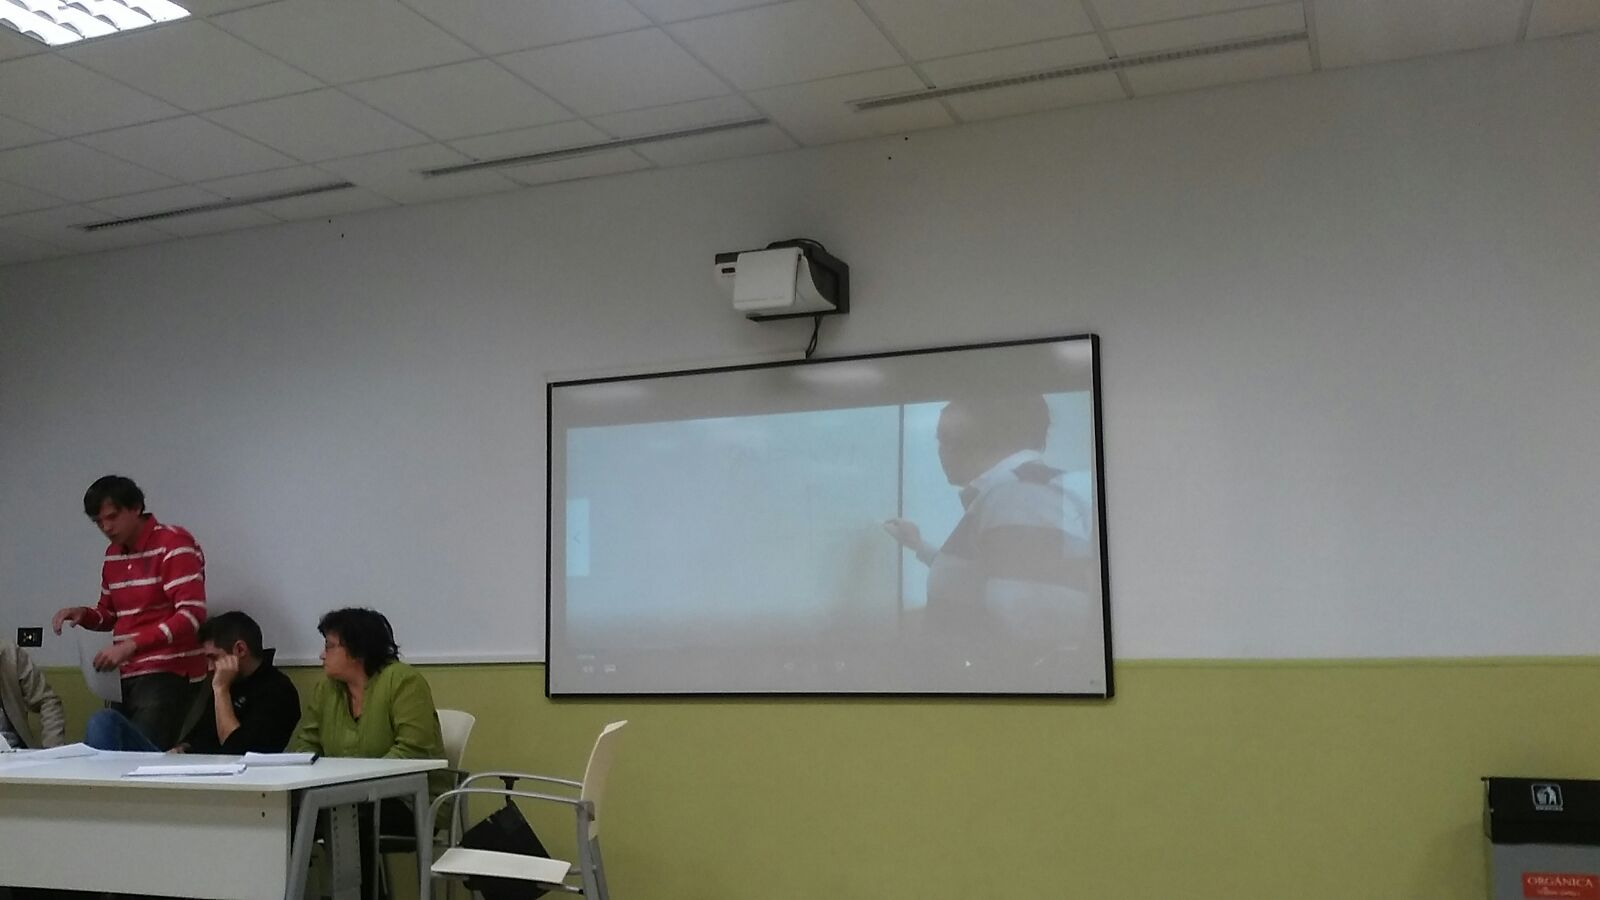
\includegraphics[scale=0.20]{img/grupo7_1.jpg}
%\caption{.}
\end{figure}

La exposición del Grupo 7 se ha basado en la metodología de “aula invertida” y un ejemplo de gamificación mediante el programa Kahoot. 

En referencia a flipped classroom, nos han explicado el procedimiento a seguir en esta metodología. El profesor sube a la red un video sobre un tema en concreto, y los alumnos visionan el video en su casa. De esta manera, las clases en el aula estarán orientadas a solucionar las dudas de los alumnos sobre la materia. Para que lo viéramos con ejemplos, los integrantes se han grabado explicando temas como representación de funciones, trigonometría, etc. En esta parte, hemos echado en falta, que nos explicaran algunos ejemplos sobre los métodos mediante los cuales el profesor se asegura que el alumno ha visionado el video antes de ir a clase. Por ejemplo, nos hubiera gustado que los videos se interrumpieras con algún tipo de pregunta que fuera necesaria responder para seguir viendo la lección o que hubieran demostrado que no se puede avanzar en la reproducción del mismo.

La segunda parte ha estado orientada a la simulación de un proceso de evaluación mediante kahoot. Esta parte nos ha gustado, porque las preguntas estaban muy bien planteadas y creemos que potenciará la competitividad entre alumnos. Lo mejor de esta aplicación está en que no solo premia si has respondido correctamente, además tu puntación es mayor si eres más rápido que tus compañeros. 


\begin{figure}[hbt]
\centering
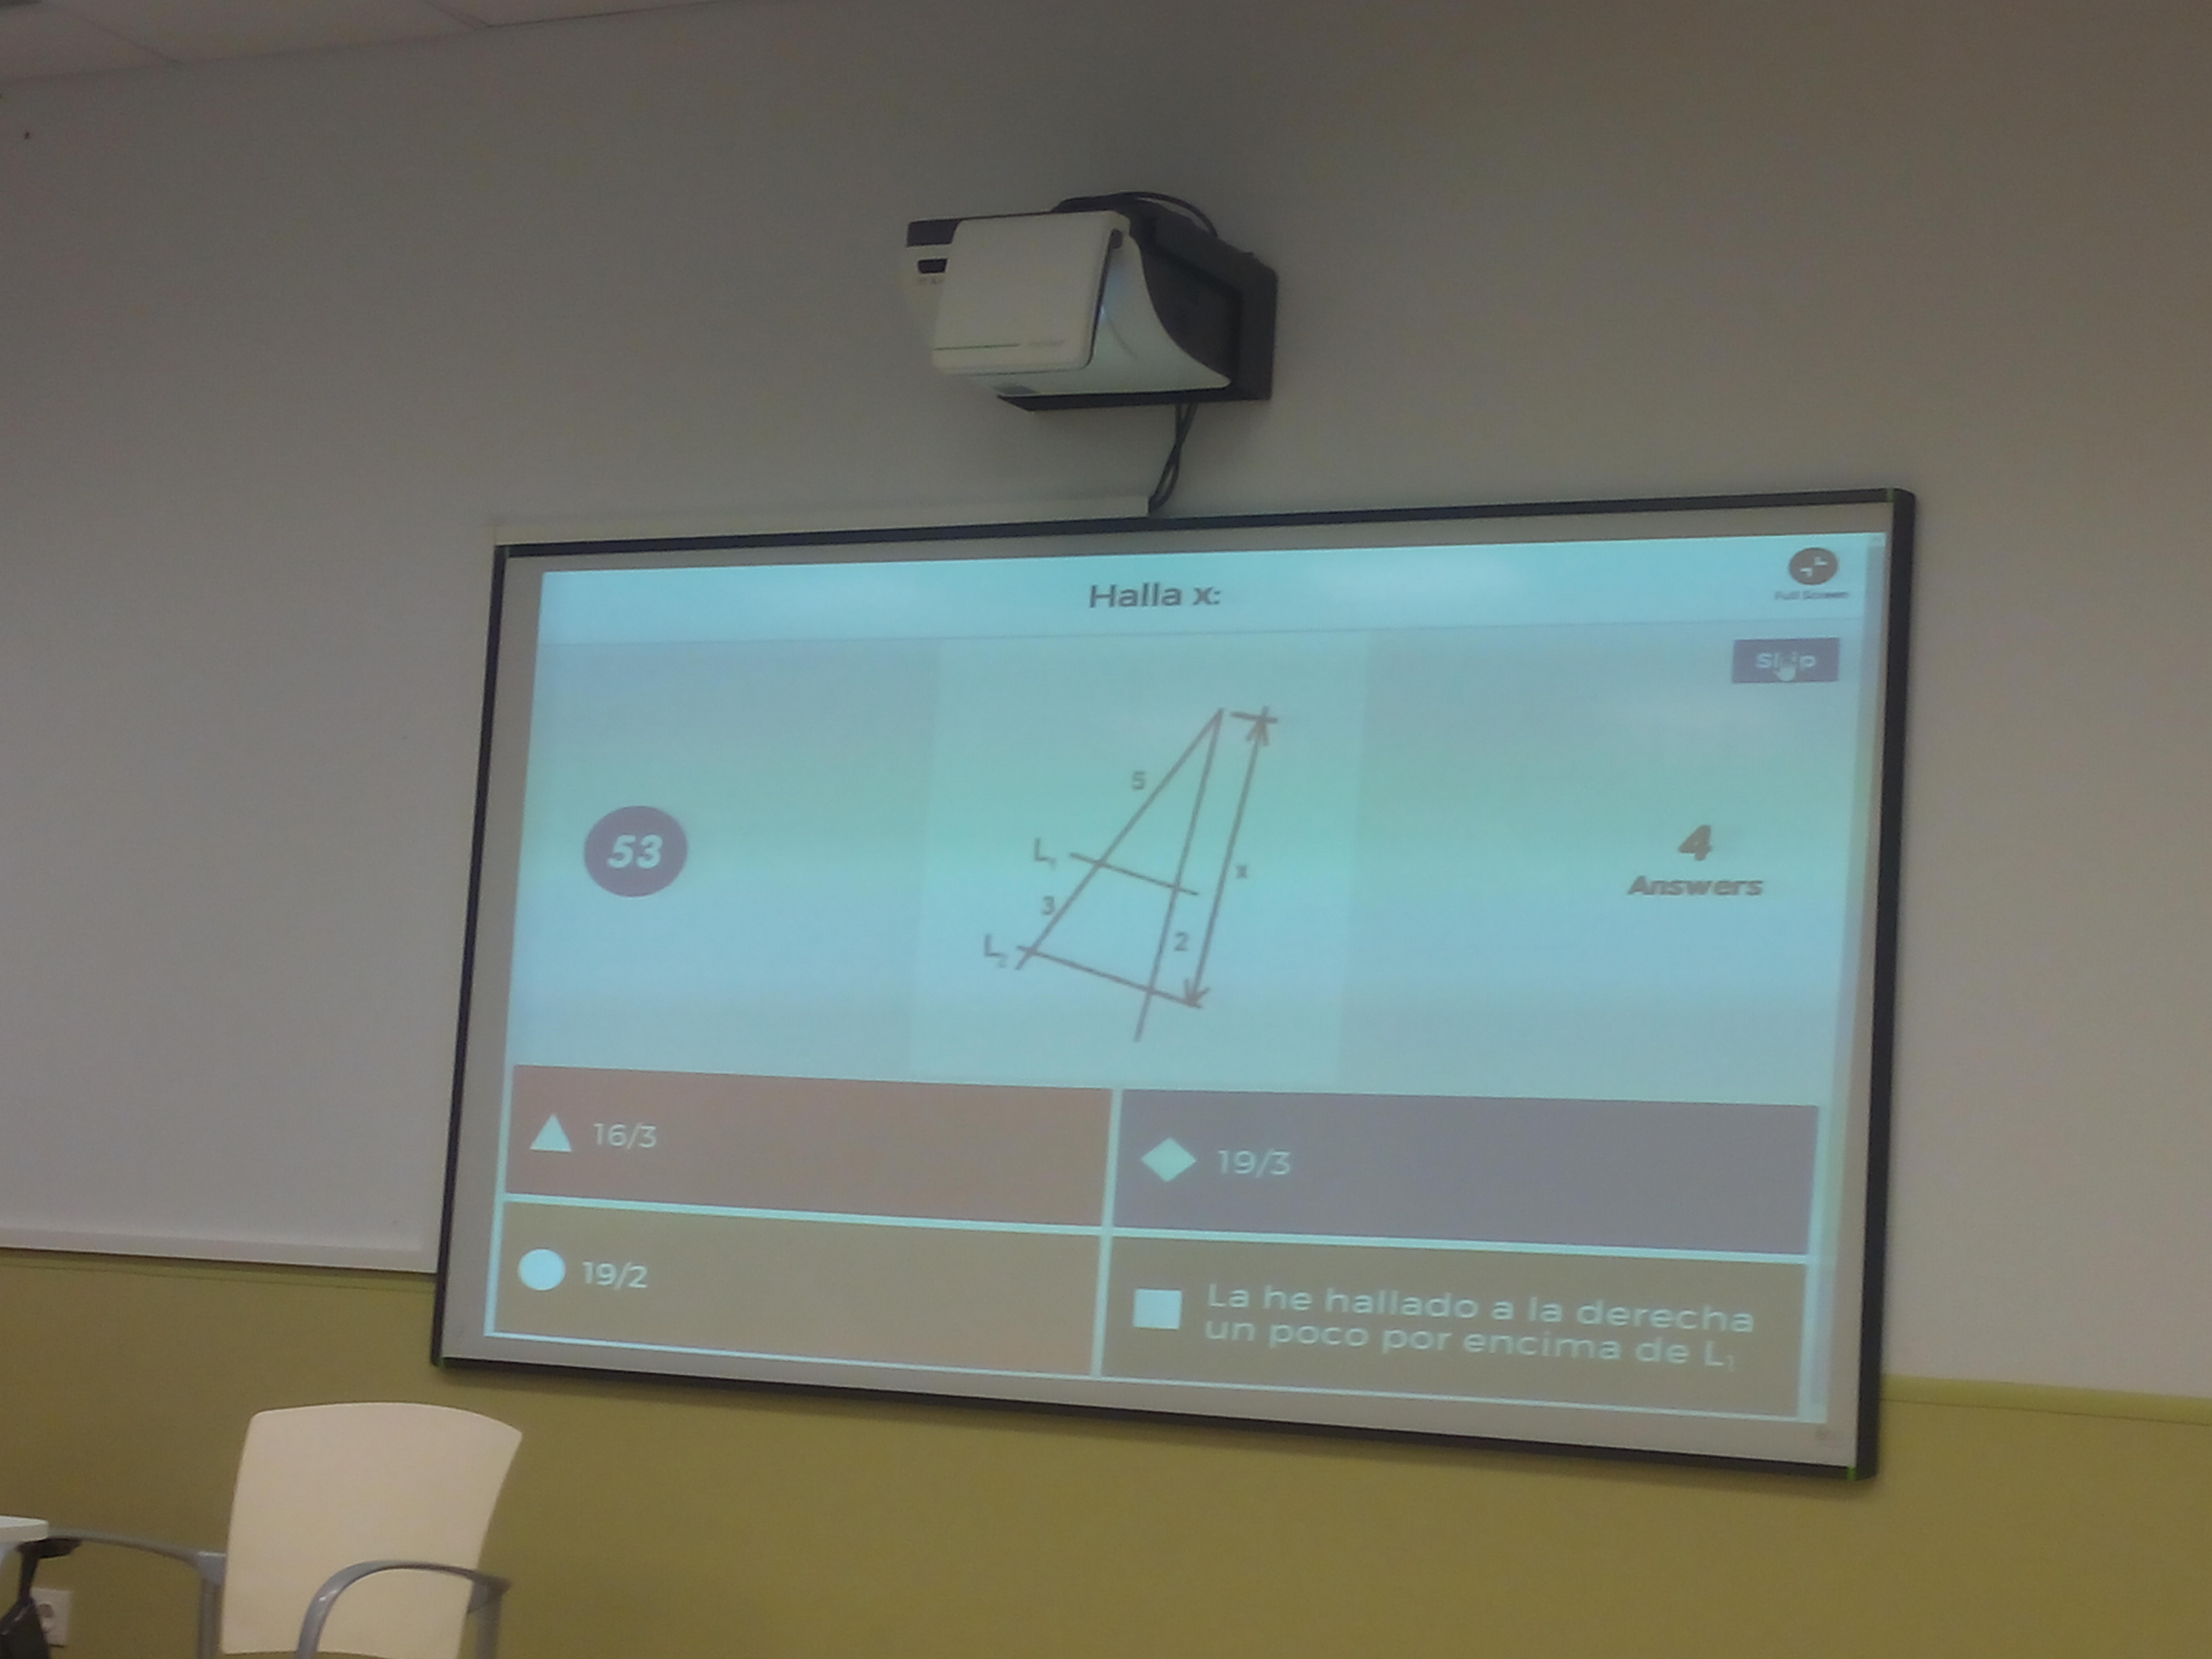
\includegraphics[scale=0.11]{img/grupo7_2.jpg}
\caption{Pregunta hecha con Kahoot sobre proporcionalidad.}
\end{figure}


Por nuestra parte, opinamos que todas estas metodologías deben ser puestas en práctica durante un período, con la finalidad de que los alumnos se vayan acostumbrando al ritmo de aprendizaje que marcan estas técnicas. Si pasado un tiempo vemos que no funcionan, podríamos ir modificando aspectos como el formato del video, la duración, utilizar otros recursos, etc.



